\section{NXTCam-v4 Sensor Analysis}\label{CamAnalysis}


\todo{Finish}

We are using the NXTCam version 4. We will be referring to it as simply the NXTCam.

The source for this section is \cite{NXTCamUserGuide}

Sensor with a high level of abstraction.

The NXTCam is a real-time image processing engine that provides high-level post-processed data of the image that the camera sees. This means it does not send the image that it can see directly to the NXT, instead it only sends data about the contents of the image. The image itself can be viewed if the NXTCam is connected directly to a computer. 

It supports two tracking modes, object tracking and line tracking.
In the context of this project, only its line tracking capabilities is useful, and as such solely the line tracking will be tested.

It can track up to 8 differently coloured objects at 30 frames per second at a resolution of 88 times 144. It returns boxes with x and y coordinates, height and width that correspond to the position of the line. While, according to the user guide, it has an image tracking resolution of 88 times 144 pixels. Although through testing it is found that the camera returns x values ranging between 0 and 176, and the y values range between 0 and 144, which seems contradictory. It does however somewhat match the dimensions that is given when taking pictures. In a more general sense, flawed, missing and incorrect documentation has plagued much of the research and experimentation with the NXTCam. 


Working with the sensor through LEGO Mindstorms should be simple. They probably have very extensive driver software and calibration. Because we're planning to use a different framework that supports real-time systems, however, we will have to write much of this ourselves. This means we have to handle much erroneous data and ensure that the bus keeps driving properly regardless. 

Citation: \cite{nxtCamDocumentation}
Data sheet and others are available for download. We've mostly been consulting the User Guide. 
Calibration by static and thorough testing, thorough testing would be very delicate, difficult and time consuming to do properly. Reason being that there are a number of different parameters that affect the NXTCam's output, some of which are very difficult to control reliably. 

For instance:
The NXTCam needs to be held completely still, otherwise it may mess up the picture by changing the parameters of the test.
The light levels need to be the same, difficult because time of day
The position of the NXTCam in comparison to the line that it should track need to be the same.

As such, the result of any measurement would only be relevant at a very specific setting, that is very difficult to recreate. 

Instead we are testing the sensor through dynamic testing to uncover errors and unexpected interactions that are there regardless of the specific setting. 


\subsection{Planning}
This is how the test is set up:
We will be conducting the test on a white background with 15 mm wide black tape marking a left turning line. Camera is placed at a height of 20 cm, it was arranged to be this high because this height gave the most correct readings of the 15 mm wide tape. The cammera will be stationary at a spot and we will take multiple results to analyse. The test will e conducted with and without yellow indoor lighting. And also check how the camera behaves while it is being shaken slightly.

Here's a birds eye view of the sensor\ref{fig:BirdsEyeView}.
\begin{figure}[H]
    \centering
    \includegraphics[width=0.5\textwidth]{Images/Analysis/NXTCamTesting/BirdsEyeView.png}
    \caption{Birds Eye View}
    \label{fig:BirdsEyeView}
\end{figure}



To conduct the tests, we used two different programs, NXTCamView and BusRemoteTool. 
NXTCamView is a program made by LEGO MINDSTORMS\copyright community member Paul Tingey to configure, view the output data from the cam and control the NXTCam sensor. 
\todo{NxtCam user manual refererer til nxtcamview, så jeg tror faktisk ikke jeg kan sige han bare er et community member}

BusRemoteTool is a program that we created ourselves to more easily see the measurements in real time, and also being able to test possible algorithms for calculating the direction that the bus should drive. There will be a more thorough description of this program in the later testing section \ref{Test:RemoteDebugging}. 

We'll use these permanent settings for colour heat map\ref{fig:CamSettings}.
\begin{figure}[H]
    \centering
    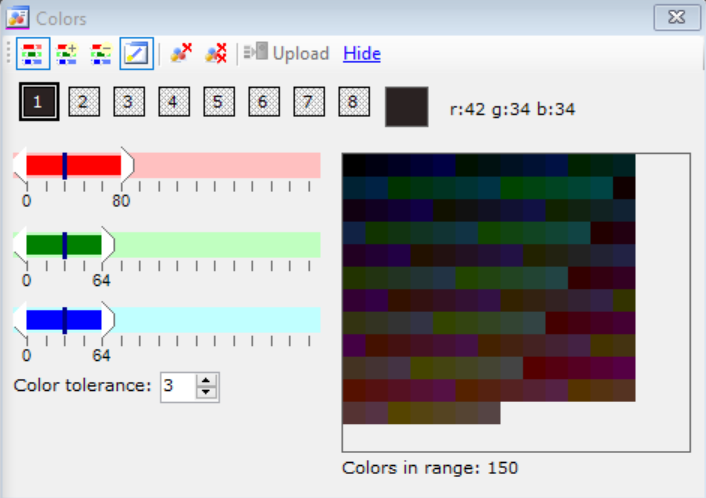
\includegraphics[width=0.5\textwidth]{Images/Analysis/NXTCamTesting/NXTCamView_ColourSettings.png}
    \caption{Camera Settings}
    \label{fig:CamSettings}
\end{figure}



We will observe the results and later perhaps adjust our design and implementation based on them.

\subsection{Results}

How the data looks as it goes through the sensor, and what it actually returns



Camera view\ref{fig:CammeraView}.
\begin{figure}[H]
    \centering
    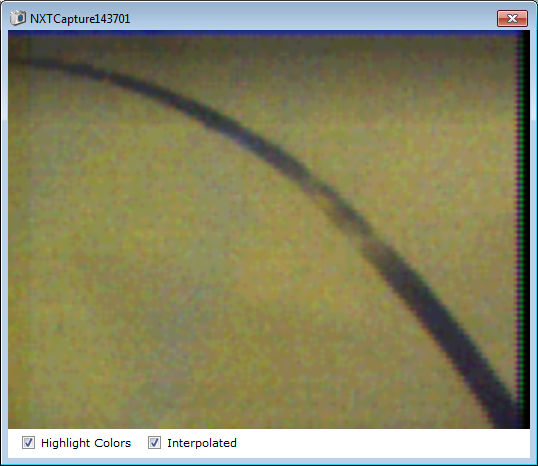
\includegraphics[width=0.48\textwidth]{Images/Analysis/NXTCamTesting/NXTCamView_Picture_NoHighlight.png}
    \caption{The view from the camera}
    \label{fig:CammeraView}
\end{figure}


%Screenshot af NxtCamView af hvad den detecter (den gul markerede linje)
What the camera marks \ref{fig:CammeraMarking}.
\begin{figure}[H]
    \centering
    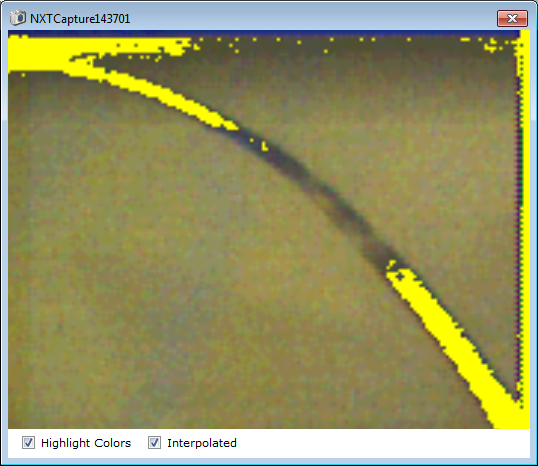
\includegraphics[width=0.48\textwidth]{Images/Analysis/NXTCamTesting/NXTCamView_Picture_Highlight.png}
    \caption{Camera marks}
    \label{fig:CammeraMarking}
\end{figure}

It's important to mark the distinction between what NXTCamView can statically measure and what the camera actually returns. These yellow markings is the data marked by the NXTCamView program, not the sensor itself. It is, however, an accurate picture of the areas that the the sensor will be likely to return as boxes. 

\subsubsection{Good Results}

Next image is a result that the sensor itself may return, and this data is what we can use in our software program. The sensor returns one of such data sets every time it is called. 
The sensor has a refresh rate of ???
Do we know how often we can ping it?

%Screenshot af NxtCamView hvor den viser os tabellen af punkterne
An illustration of the data received generated by NXTCamView\ref{fig:CamOutput1} when it goes well.
\begin{figure}[H]
    \centering
    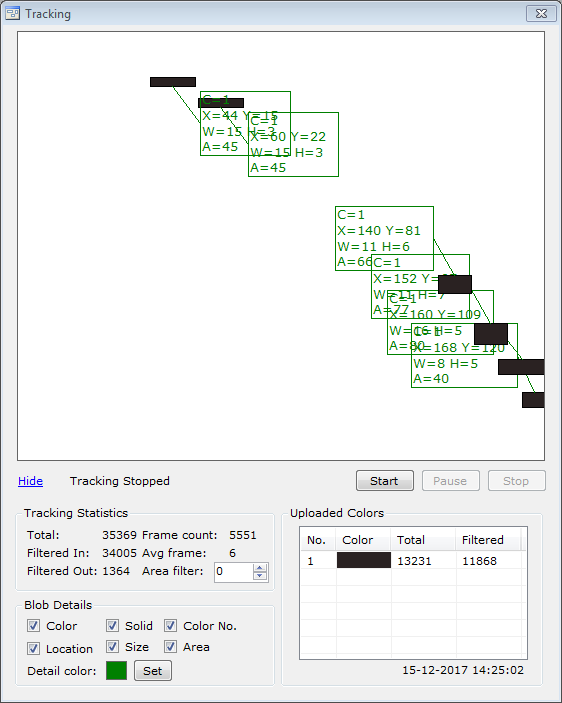
\includegraphics[width=0.48\textwidth]{Images/Analysis/NXTCamTesting/NXTCamView_Boxes_1.png}
    \caption{Camera Output}
    \label{fig:CamOutput1}
\end{figure}

Now we've taken the data returned from the sensor and plugged it into our own testing program, the BusRemoteTool, where it is even easier to see how the data points look.

%Screenshot af BusRemoteTool, hvor vi bare ser punkterne
RemoteTool illustration of a output from the camera in Figure\ref{fig:RemoteToolOutput1}. In this Figure the size and location of boxes and not the colour is important. Also disregard the red line.
\begin{figure}[H]
    \centering
    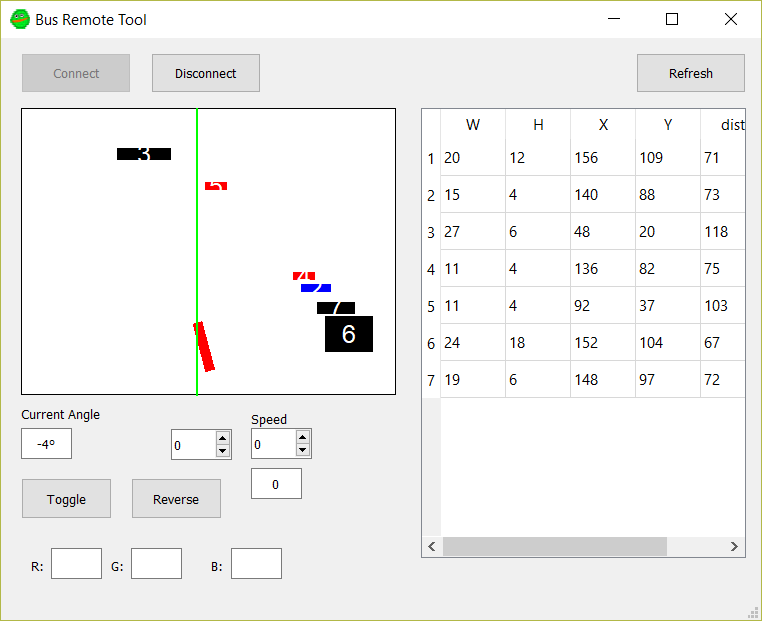
\includegraphics[width=0.48\textwidth]{Images/Analysis/NXTCamTesting/BusRemoteTool_Good.png}
    \caption{Example of an output illustrated in RemoteTool}
    \label{fig:RemoteToolOutput1}
\end{figure}

%Se bort fra farver og stregen på billedet: de er ikke vigtige for denne test. 



\subsubsection{Bad Results}
Nevertheless, the NXTCam is a sensor like the rest, and it will not always deliver useful data. 

Screenshot af NxtCamView, hvor vi ser punkterne og det går galt
Figure \ref{fig:RemoteToolOutput2} is a Illustration of an example of an output in RemoteTool, where the output does not correspond to the line 
\begin{figure}[H]
    \centering
    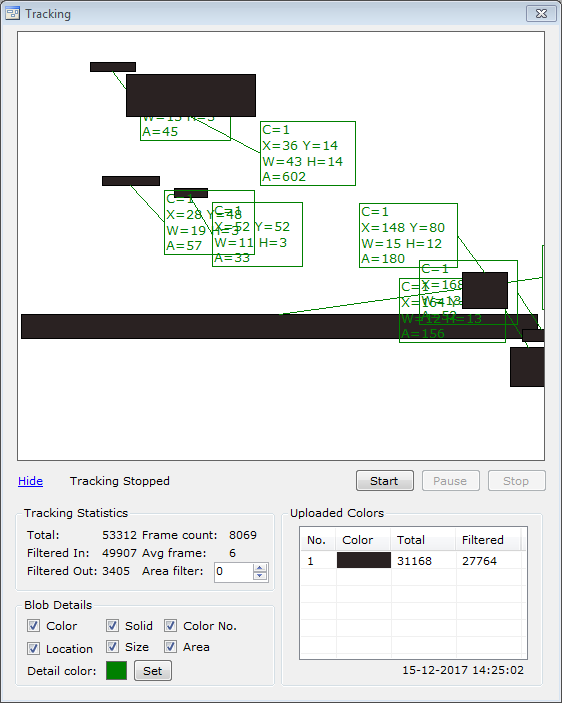
\includegraphics[width=0.48\textwidth]{Images/Analysis/NXTCamTesting/NXTCamView_Boxes_2.png}
    \caption{Example of incorrect output illustrated in RemoteTool}
    \label{fig:RemoteToolOutput2}
\end{figure}



Similarly, In Figure \ref{fig:RemoteToolOutput3} from BusRemoteTool where it also goes wrong. Here there are very few boxes. The rest were simply not returned by the sensor this time. Note, it's still placed at the same spot with the same conditions as previously.
\begin{figure}[H]
    \centering
    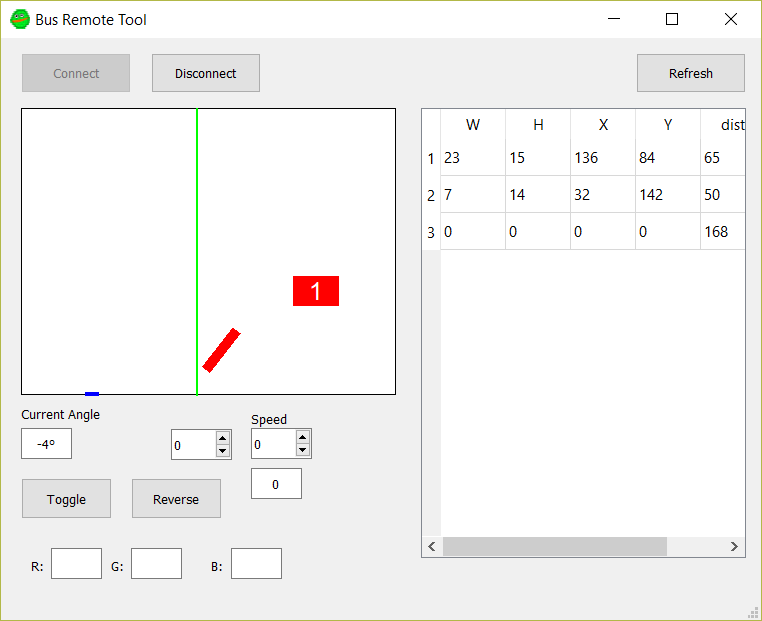
\includegraphics[width=0.48\textwidth]{Images/Analysis/NXTCamTesting/BusRemoteTool_Few.png}
    \caption{Another example of incorrect output illustrated in RemoteTool}
    \label{fig:RemoteToolOutput3}
\end{figure}



In Figure \ref{fig:RemoteToolOutputZero} an example of Zero Boxes are illustrated.
\begin{figure}[H]
    \centering
    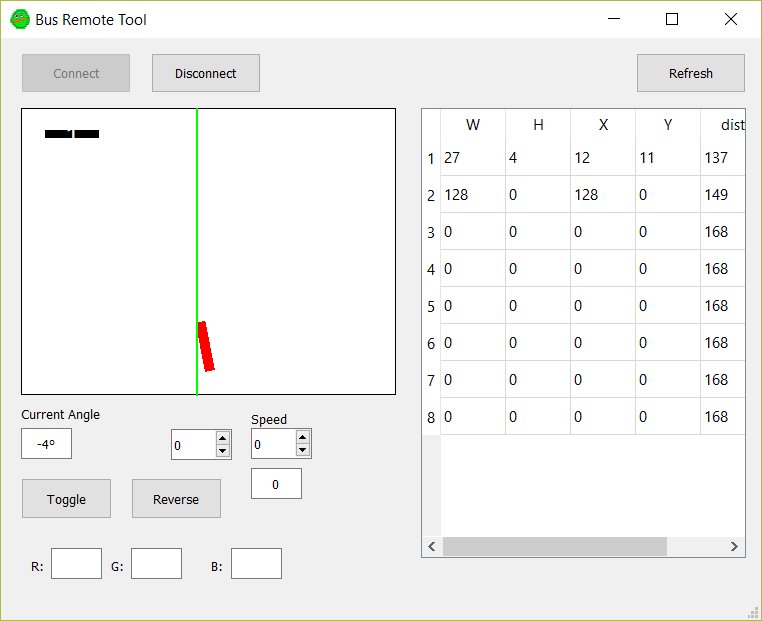
\includegraphics[width=0.48\textwidth]{Images/Analysis/NXTCamTesting/BusRemoteTool_ZeroBoxes3.png}
    \caption{An example of zero boxes}
    \label{fig:RemoteToolOutputZero}
\end{figure}



In Figure \ref{fig:RemoteToolMassive} an example of a random Big Box.
\begin{figure}[H]
    \centering
    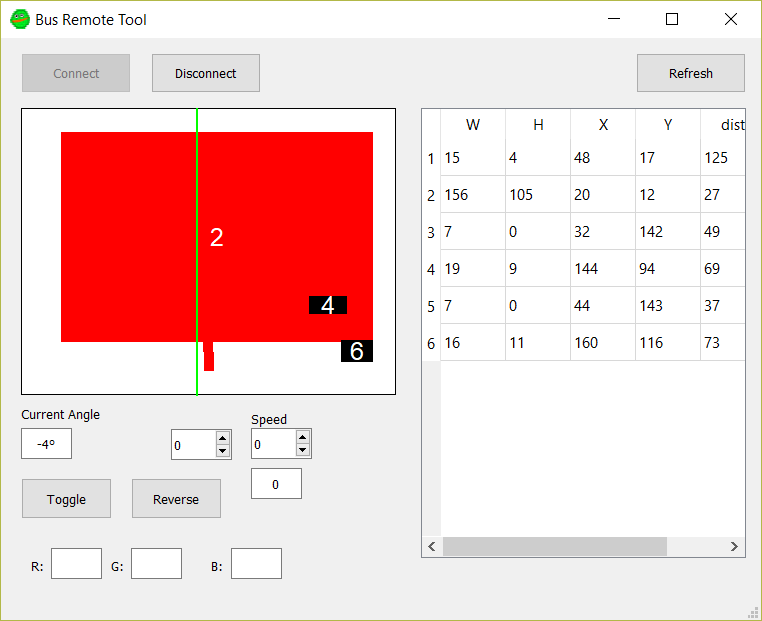
\includegraphics[width=0.48\textwidth]{Images/Analysis/NXTCamTesting/BusRemoteTool_BigBox.png}
    \caption{An example of an incorrect output with a massive Box}
    \label{fig:RemoteToolMassive}
\end{figure}

\subsubsection{Dim Light Source}
We slowly pulled the platform upon which the sensor was placed and line was marked into an unlit corridor. No picture of this test is provided as camera lighting correction software makes it tough to illustrate which lighting situation we were in. 

We expected that there would be large dark boxes that covered the shadowy areas of the measured area, covering a larger area depending on how dark the room was. In situations lit only slightly less than in the previous tests, the boxes would favour the area where line went, and as it got darker, it would slowly stop favouring the line, and just mark shadowy areas.

In our tests, however, it did not stop favouring the line in a slow fashion. Instead, within only a slight difference in lighting, the boxes stopped favouring the position of the line at all, and instead filled the most shadowy areas. It was much more of an either-or situation than what we expected; either the lighting was enough to detect the line, or it was not. 

As we were curious to see which data it would return on the threshold between detecting the line and not doing so, we did additional tests at this position. We found that while the lane was still somewhat consistently detected, large bars were now shown regularly. These bars were inconsistent in height, but always the width of measured area, and they favoured the shadowy areas. 

\todo{}



\subsubsection{Shaking Camera}
Tilting the sensor tower from left to right. 
We expected more erratically positioned and smaller boxes, as well as more zero boxes.
Instead we found that it did not affect the results in any noticeable way. Presumably the accuracy of the box positions still declined, but we did not encounter enough evidence to conclude this. While we could have done statistical analysis to decide this for sure, we chose not to. 
Reason being, we were shaking the camera very heavily to provoke a result, and far more than any LEGO bus would ever be able to do. If we didn't cause any major issues, then the shaking of the bus would not do either. Irregardless of the specific accuracy, any algorithm to drive the bus would still have to contend with erratic data, regardless of shaking or not. We concluded that erratic data cannot be countered by making the camera sit in a stable position.

\todo{Sæt noget af dette ned i konklusionen}

\section{Other Points of Note} \todo{Can we find a better title?}\label{noteworthyCam}
While experimenting with the sensor, we encountered a number of noteworthy interactions, many of which we need to consider during the implementation for the sensor to work. 



%Vi havde problemer med at den altid returnerede 8 objekter, selv hvis der ikke var 8 objekter
There was a problem where the sensor would without exception return 8 boxes when in line mode. Some of these boxes would be of height and width 0 meaning they mark an area of 0. Since their area is 0 the NXTCam is saying that i see nothing in that spot however still marking it as a box, which is useless information. However, after a weekend of disuse it suddenly were able to return less than 8 boxes. It would still return some "0 boxes" but consistently until reaching the 8 boxes. 
%Der var et ikke-reproducbart problem med at den kunne blive stuck i line mode

There was a problem where we had trouble sending the settings to the sensor. We were unable to send the settings from the NXT Brick to the sensor. We had a workaround by sending the setting from a computer to the sensor by using NXTCamView. Through the workaround, we concluded that the problems were not stemming from the internals of the sensor. However, this error also suddenly stopped occuring in the sensor after a weekend of disuse.

%Fejl 78 er miskonfigureret (fx ikke sortering til før man sætter den i line mode), men man har ikke brug for sortering før man sætter den i object mode

Another problem that took a while to resolve was that instead of sending data about the boxes that make up the line that the sensor was supposed to track, the sensor would return the integer number "78". However, the boxes shown in the NXTCamView were correct, and when set in the object mode it sent the actual data to the NXT Brick. Since knew the sensor found the correct boxes we concluded the sensor were working, and it had to be a problem with the communication between the NXT Brick and the sensor. We then consulted the NXTCam data sheet, to figure out what "78" could mean; however, we were unable find any information in the data sheet. It was resolved by a forum post that informed us that an object count of "78" meant configuration error. The error was resolved by calling the sort-function prior to use in Line Mode. We used \code{camera.sendCommand('X');} which is the command for no sorting. 

%This meant that we could look at the actual data within the NXTCamView, however the NXT brick would only be given integer "78". 



\section{Conclusion}

The sensor is somewhat of a black box, difficult to diagnose problems and find solutions, because we do not know where something went wrong. We have concluded the following large causes for faulty data. 

Sensitive to light (and shadows, so watch where you're standing)
Sensitive to movement
Often seemingly random boxes with seemingly random size

So this means:
Inconsistent data
A single measurement is unreliable
Nevertheless, multiple measurements approximate the line 

So to use the data from the NXTCam in further work and produce the most consistent results, the following things are necessary: 
We need a consistent light source 
Algorithms need to use multiple measurements and/or the algorithm should not be able to turn the bus based on only few measurements. So perhaps it should turn the bus incrementally in stead of immediately. 



Very high level of abstraction, and inherently supports line tracking functionality which would be really useful to solve our requirement of staying within one road lane. To use it in our product we need to write some software that sorts out bad measurements like the large bars, very large boxes and zero boxes. 
Unless we do this incredibly well, we need an algorithm that uses multiple measurements and or only turns the bus incrementally. 
Also we need to assume bright and even lighting conditions.